%% Tasks for Proposed Solution

In order to implement and analyze the proposed solution, work has been broken
down into three phases: the implementation phase, the testing phase, and the
report phase. The implementation phase focuses on doing initial benchmarking and
developing of the proposed daemons. The testing phase will consist of analyzing
the data that is generated from the implementation phase. The report phase is
where the final report and presentation are created and all of the results
summarized. 

\begin{figure*}[ht]
    \centering
    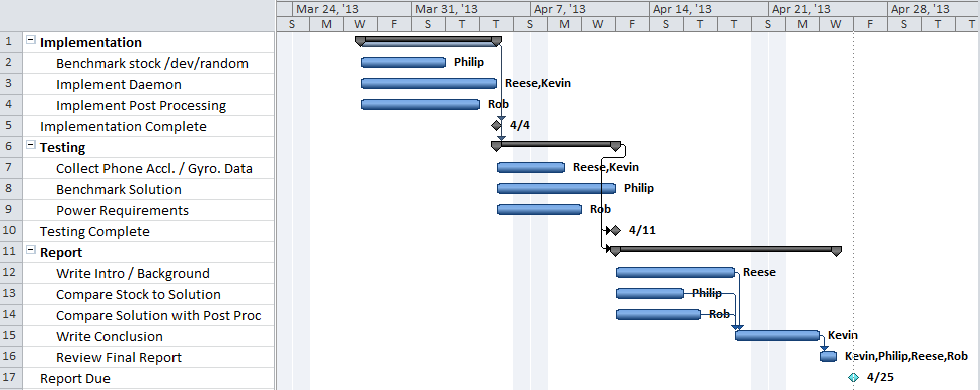
\includegraphics[scale=0.71]{proj-ghantt-v3}
    \caption{Assigned tasks and estimated time of completion}
    \label{fig:gahntt}
\end{figure*}

The work timeline is layed out on the Ghantt chart in Fig.~\ref{fig:gahntt} on
page \pageref{fig:gahntt}. This chart shows who will be performing which tasks,
and when they will begin and finish those tasks. It also shows how the stages
are dependent upon the previous stage being completed. Breaking down the tasks
like this helps the project move forward at a reasonable and planned pace.

In the implementation phase of the project, one member of the group will
benchmark existing randomness sources on the board in order to generate a
baseline against which any developed randomness solution can be measured. Two
members of the project will develop the daemon discussed earlier to take
presumably random data from the accelerometer and introduce it into the entropy
pool of the Linux kernel. One member of the group will develop several post
processing implementations which will hook into the daemon to provide better
entropy to the kernel than simply taking all of the raw data. Most of the
development will be done in this phase of the project, as the rest of the
project will be focused on collecting and analyzing data and building the
conclusions for the final report.

The testing phase of the project is where data will be collected using the
solution developed in the implementation phase. Two members of the group will
collect accelerometer and gyroscope data for later analysis, to show that this
data has consistent properties. As a development platform, the Dragonboard is
not intended to be carried on a person, as a traditional cellphone would be.
This means that the team members collecting data will not only collect data on
the board, to show the effects of relative stillness on the sensors, but also
collecting data on personal cellphones. This will require some analysis to show
that these tests properly approximate what they would have been using a mobile
Dragonboard. The member of the project who benchmarked the stock randomness
solution will now follow a similar procedure to benchmark the developed
solution. This will allow for direct comparison between the stock and developed
solutions, showing what benefit the developed solution provides. A member of the
project will benchmark the developed system in terms of its power draw, running
the system while sampling the current draw of the entire system, to show the
effects that this implementation has on the battery life of the device.

During the review phase of the project all of the data will be analyzed so that
the final report and presentation can be prepared. The entire paper will be
split between all of the members of the project. It is partitoned in such a way
that the members are writing the sections that they would have had most exposure
to during the initial two phases of the project. After indvidual contributions
have been made, the group will meet as a whole to discuss the paper, including
finalizing the conclusion. This will culminate with submitting the deliverables.

